\chapter{Problemanalyse}
    Kapitel \ref{chapter:introduction} ist nur einleitend
    auf die Problemstellung dieser Arbeit eingegangen.
    Eine ausführlichere Betrachtung folgt in diesem Kapitel.
    Dazu wird zunächst die Problemdomäne erläutert.
    Es folgt die Vorstellung der Content Management Systeme,
    die sich an der {\fernUni} im Einsatz befinden
    und wie eine manuelle Migration von einem System zum anderen
    ablaufen kann.
    Basierend auf diesen Ausführungen wird anschließend
    die Herausforderung und die resultierende Problemstellung
    detailliert diskutiert.

    \label{chapter:ProblemAnalysis}
    \section{Das World Wide Web}
    \label{section:TheWWW}
    % TODO Keine umfassende Betrachtung, da zu viel. Nur Aspekte, die für Arbeit wichtig.
    Zur Lösung der beschriebenen Problemstellung ist eine genauere
    Betrachtung ihrer Domäne notwendig.
    Das Problem wird dadurch in einen größeren Kontext gesetzt,
    was zu einem besseren Verständnis und damit zur Findung
    einer geeigneten Lösung beiträgt.
    % TODO: Ref auf DDD?

    Die in diesem Fall zu betrachtende Domäne ist das "`\gls{www}"'.
    Diese wird im Folgenden aus zwei Perspektiven betrachtet:
    Zunächst wird die Sicht eines Webseitenbesuchers auf das \gls{www} beschrieben.
    Anschließend stehen die konzeptionellen und technischen Grundlagen
    des \gls{www} im Vordergrund.
    Zusammen vermitteln diese Erläuterungen hinreichendes Wissen,
    um eine Lösung für die gegebene Problemstellung zu erarbeiten.

    \subsection{Das World Wide Web für Webseitenbesucher}
        \label{section:enduserViewOnWWW}
        Die Sicht eines Webseitenbesuchers (im Folgenden auch "`Endnutzer"' genannt)
        auf das \gls{www} ist simpel und sollte von jedem Leser nachvollzogen werden können.
        Dennoch bietet sie wichtige Einblicke.

        \paragraph*{Der Browser}
        Zugang zum \gls{www} erhält ein typischer Endnutzer über einen \textit{Browser}.
        In dessen Adresszeile trägt er einen \gls{url} ein,
        woraufhin der Browser die gewünschte Webseite lädt und anzeigt.
        Eine Webseite ist aus Sicht eines Endnutzers also eindeutig über eine
        Adresse, die allgemein "`URL"' oder "`Link"' genannt wird, gekennzeichnet.
        Der Browser dient zur Anzeige von Webseiten, wodurch er für Webseitenbesucher
        zu einem unentbehrlichen Werkzeug wird.
        Browser existieren für verschiedene Endgeräte,
        wie PCs, Smartphones und Tablets.
        Das heißt ein Webseitenbesucher ist nicht an eine Form von Endgeräten gebunden.

        \paragraph*{Bestandteile}
        Sieht sich ein Besucher eine Webseite im Browser an,
        kann er schnell verschiedene Bestandteile ausmachen.
        Dazu zählen zunächst simple Elemente, mit denen er wenig bis gar nicht
        interagieren kann, also statischer Natur sind.
        Vertreter dieser Gruppe sind

        \begin{itemize}
            \item Texte,
            \item Bilder,
            \item Videos,
            \item Links auf andere Webseiten und
            \item Dateien, die zum Download bereitstehen.
        \end{itemize}

        Des Weiteren besitzt eine Webseite Designelemente,
        die in ihrem Aufbau oder ihrer Funktion komplexer
        als die zuvor genannten sind.
        Die Bibliothek Bootstrap\footnote{https://getbootstrap.com/}
        enthält zahlreiche solcher Komponenten.
        Beispielsweise bietet die Komponente "`Card"' die Möglichkeit
        Inhalte in komplexe Behälter einzubetten \cite{bootstrap:Cards}.
        Ein anderes Beispiel ist die Komponente "`Carousel"',
        welche der Erstellung von Diashows dient \cite{bootstrap:Carousel}.
        Letztere und viele weitere bieten dem Nutzer
        erweiterte Möglichkeiten zur Interaktion mit einer Webseite.

        Das gilt auch für Formular- oder Steuerelemente,
        die aus klassischen Applikationen bekannt sind,
        aber auch in Webseiten Anwendung finden.
        Dazu gehören unter anderem

        \begin{itemize}
            \item Textfelder,
            \item Schaltflächen,
            \item Dropdown-Listen,
            \item Checkboxen und
            \item Radiobuttons.
        \end{itemize}

        Allen Elementen ist gemein, dass ihr Aussehen sich von
        zwischen verschiedenen Webseiten unterscheiden kann.

        \paragraph{Varianten}
        Aus Sicht eines Endnutzers existieren oftmals mehrere
        Varianten derselben Webseite.
        Welche Variante er sieht hängt dabei von zwei Dimensionen ab:
        Sprache und Endgerät.

        Die heutige globalisierte und vernetzte Welt machen es oft erforderlich
        einen Internetauftritt auch auf internationele Besucher vorzubereiten.
        An erster Stelle bedeutet dies, dass Inhalte in verschiedene Sprachen
        übersetzt werden, um sie einem möglichst großen Publikum zugänglich zu machen.
        Für einen Endnutzer gibt es prinzipiell zwei Methoden,
        wie er eine Seite in seiner favorisierten Sprache anzeigen kann:

        \begin{itemize}
            \item   Die Webseite bietet ihm ein Steuerelement,
                    über das er selbst eine Sprache auswählen kann.
            \item   Die Webseite ermittelt automatisch die geeignete Sprache,
                    anhand verschiedener Parameter, die für den Besucher nicht zwangsläufig
                    offensichtlich sind.
        \end{itemize}

        Die Popularität mobiler Endgeräte wie Smartphones und Tablets
        bewegt immer mehr Betreiber von Webseiten dazu,
        verschiedene Versionen ihres Internetauftrittes anzubieten,
        die für verschiedene Geräte optimiert sind.
        Aus Sicht eines Besuchers gibt es bis zu drei geräteabhängige
        Varianten einer Webseite. Zwei für die oben genannten mobilen Geräte
        sowie eine weitere für PCs.
        Für ihn sind dabei drei Unterscheidungsmerkmale dieser Varianten offensichtlich:
        Inhalt, Design und Funktionalität.
        Ziel jeder Maßnahme ist es die Anzeigefläche,
        die ein Endgerät bietet, sinnvoll zu nutzen.
        Je kleiner ein Gerät ist, desto geringer ist diese Fläche,
        weshalb Inhalte auf kleineren Geräten weggelassen oder anderes
        dargestellt werden.
        Genauso können gewisse Funktionen einer Webseite nicht gleich
        gut sowohl auf großen PC- als auch auf kleinen Smartphone-Displays
        umgesetzt werden, ohne Anpassungen vorzunehmen.
        
        \paragraph*{Webanwendungen}
        Kapitel \ref{section:ContentManagementAndDesign} hat bereits
        kurz aufgezeigt, wie sich Webseiten stets weiterentwickeln.
        Ein wichtiger Aspekt dieser Weiterentwicklung ist aus Sicht
        eines Webseitenbenutzers, wie stark er mit ihr interagieren kann,
        was schon im Abschnitt über die Bestandteile einer Seite kurz aufgegriffen wurde.

        Angefangen bei simplen Seiten,
        die ursprünglich lediglich dazu gedacht waren Informationen
        bereitzustellen und mit anderen zu
        verlinken \cite{bernersLee:InformationManagement},
        entwickelten sich Webseiten im Laufe der Zeit weiter
        und boten immer mehr Möglichkeiten mit dem Nutzer zu interagieren
        und auf seine Aktionen zu reagieren.
        Folglich hielten immer mehr Merkmale klassischer Computeranwendungen
        Einzug in Webseiten.
        Heute stehen Webseiten klassischen Applikationen in Nichts nach,
        weshalb mit ihnen auch komplexe Anwendungen umgesetzt werden.
        Ein gutes Beispiel hierfür sind Googles Office-Anwendungen
        Docs\footnote{\url{https://www.google.com/intl/de/docs/about/}},
        Sheets\footnote{\url{https://www.google.com/intl/de/sheets/about/}},
        und Slides\footnote{\url{https://www.google.com/intl/de/slides/about/}},
        die in der Lage sind in vielen Fällen klassische Office-Anwendungen zu ersetzen.
        Aufgrund dieses besonderen Charakters ist für solche Webseiten auch der Begriff
        "`Webanwendung"' gebräuchlich.

        Im Vergleich zu herkömmlichen Anwendungen besitzen Webanwendungen zwei wichtige Vorteile.
        Solange man einen Internetzugang hat, sind sie zu jeder Zeit und von jedem Ort aus nutzbar.
        Des Weiteren können sie auf jedem Gerät ausgeführt werden,
        das einen Browser besitzt. Wie zuvor beschrieben ist dies nicht mehr ausschließlich ein PC,
        sondern auch mobile Endgeräte wie Smartphones und Tablets.

        \paragraph*{Websites}
        Der Internetauftritt einer Organisation besteht selten aus einer
        einzelnen Webseite.
        Stattdessen besteht er aus vielen Webseiten,
        die untereinander verlinkt sind und von der jede einen eigenen
        \gls{url} besitzt.
        Neben "`Internetauftritt"' hat sich der Begriff "`Website"' zur
        Referenzierung dieser Gesamtheit aller Webseiten einer Organisation
        etabliert \cite{duden:Internetauftritt, oxford:Website}.

        \paragraph*{Klassifizierung}
        Basierend auf ihrer primären Funktion lassen sich Webseiten grob klassifizieren.
        Die Bezeichnungen der resultierenden Klassen finden sich häufig im Sprachgebrauch
        von Webseitenbesucher wieder.

        Die Seiten \url{https://www.google.de} und \url{https://www.bing.com/}
        werden beispielsweise häufig als \textit{Suchmaschinen} bezeichnet.
        Andere geläufige Klassen sind:

        \begin{itemize}
            \item Online-Shops,
            \item Blogs,
            \item Homepages (Internetauftritt einer Organisation oder Privatperson),
            \item Social Networks
            \item Wikis
        \end{itemize}

        Eine weitere Kategorie sind die bereits erörterten Webanwendungen,
        also Webseiten, die bewusst als Oberflächen vob Anwendungen wahrgenommen werden.

        Viele Webseiten können unterschiedlich klassifiziert werden.
        Jede Suchmaschine und jeder Online-Shop ist gleichzeitig auch eine
        Webanwendung. Wie am Anfang dieses Abschnittes erwähnt ist für die
        Klassifizierung aus Endnutzersicht aber die primäre Funktion einer Webseite
        relevant.

    \subsection{Konzeptionelle und technische Grundlagen}
        Nach der Sicht eines Endnutzers auf das \gls{www},
        folgt in diesem Kapitel eine Erläuterung der Konzepte und Grundlagen,
        auf denen es basiert.

        \paragraph*{Definition des \glspl{w3c}}
        Das \gls{w3c} definiert den Begriff "`World Wide Web"' in \cite{w3c:wwwArch} wie folgt:

        \begin{quote}
            The \textit{\textbf{World Wide Web}} (\textit{\textbf{WWW}}, or simply \textit{\textbf{Web}})
            is an information space in which the items of interest, referred to as resources,
            are identified by global identifiers called Uniform Resource Identifiers (\textit{\textbf{URI}}).
        \end{quote}

        Darüber hinaus nennt \cite{w3c:wwwArch} die drei grundlegenden Komponenten des \gls{www}:

        \begin{quote}
            They are identification of resources,
            representation of resource state, and the protocols
            that support the interaction between agents and resources in the space.
        \end{quote}

        \paragraph*{\resources}
        Aus der obigen Definition wird deutlich,
        dass das \gls{www} nicht ausschließlich zur Nutzung von Webseiten
        vorgesehen ist.
        Stattdessen können über das \gls{www} jede Art von {\resources} bezogen werden.
        Neben Webseiten gehören dazu unter anderem auch einfache Textdateien
        und Binärdateien wie zum Beispiel PDFs, Audio- oder Videodateien.

        \paragraph*{Identifizierung von \resources}
        Die Beschreibung des \glspl{w3c} stellt außerdem klar,
        dass {\resources} nicht ausschließlich über \glspl{url} angesprochen werden können.
        Stattdessen geschieht dies über \glspl{uri}, die eine Obermenge von \glspl{url} darstellen
        \cite[Kapitel 1.1.3, Seite 7]{rfc:3986}.
        Jede {\resource} im \gls{www} wird also eindeutig über eine \gls{uri} identifiziert.

        \paragraph*{Interaktion mit dem \gls{www}}
        Wie in Kapitel \ref{section:enduserViewOnWWW} beschrieben ist für Endnutzer
        der Browser das einzige Werkzeug, mit dem sie mit dem \gls{www}
        interagieren können. Wie bereits klargestellt wurde,
        können aus dem \gls{www} allerdings nicht nur Webseiten bezogen werden,
        weshalb es naheliegend ist, dass neben Browsern noch weitere Werkzeuge existieren,
        um {\resources} im \gls{www} anzusprechen.
        Das \gls{w3c} bezeichnet jedes Werkzeug, das dazu in der Lage ist, als
        "`Web agent"' und beschreibt diese Rolle wie folgt:
        "`A person or a piece of software acting on the information
        space on behalf of a person, entity, or process."' \cite[Kapitel 6]{w3c:wwwArch}.
        Eine Spezialisierung stellen die sogenannten "`User agents"' dar,
        die das \gls{w3c} als "`One type of Web agent;
        a piece of software acting on behalf of a person."' beschreibt \cite[Kapitel 6]{w3c:wwwArch}.
        Browser sind User agents, aber zum Beispiel auch Kommandozeilenprogramme
        wie curl\footnote{https://curl.haxx.se/}.
        Ihre persönliche Kennung halten User Agents zum Beispiel im
        HTTP-Header "`User-Agent"' fest \cite[Kapitel 5.5.3, Seite 46]{rfc:7231}.

        Der Prozess, bei dem ein Agent über eine \gls{uri} auf eine {\resource}
        zugreift heißt "`Dereferencing the URI"' \cite[Kapitel 3.1]{w3c:wwwArch}.
        Wie dieser Prozess aussieht hängt von der Funktion des User Agents und der \gls{uri} ab
        \cite[Kapitel 3.1]{w3c:wwwArch}.
        Die Funktion eines User Agents könnte beispielsweise das Abrufen einer
        Repräsentation der {\resource} vorsehen, wohingegen ein anderer Agent
        lediglich prüft, ob eine eben solche Repräsentation existiert.
        Das Schema einer \gls{uri} beschreibt laut Spezifikation
        lediglich, wie die folgende Kennung zu interpretieren ist
        \cite[Kapitel 3.1, Seite 17]{rfc:3986}.
        Viele Schemata sind allerdings nach Protokollen benannt,
        weshalb sie in der Praxis häufig bestimmen,
        wie User Agents auf eine {\resource} zugreifen können
        \cite[Kapitel 3.1]{w3c:wwwArch}.
        
        Schemata, die im \gls{www} häufig Anwendung finden,
        sind zum Beispiel
        http\footnote{\url{https://tools.ietf.org/html/rfc7230\#section-2.7.1}},
        https\footnote{\url{https://tools.ietf.org/html/rfc7230\#section-2.7.2}},
        mailto\footnote{\url{https://tools.ietf.org/html/rfc6068}} und
        data\footnote{\url{https://tools.ietf.org/html/rfc2397}}.
        Für Webseiten sind dabei vor allem http und https
        und die gleichnamigen Protokolle von Bedeutung,
        da \glspl{url} von Webseiten diese vorrangig verwenden.

        Wenn ein Browser oder ein anderer Agent eine Webseite aufruft,
        bedeutet dies allgemein gesprochen, dass der Agent eine Repräsentation
        einer {\resource} anfragt, die er über eine \gls{url} spezifiziert.
        Konkret richtet er diese Anfrage an einen Server,
        wozu er das Protokoll HTTP(S)\footnote{\url{https://tools.ietf.org/html/rfc7231}} und die Methode
        GET\footnote{\url{https://tools.ietf.org/html/rfc7231\#section-4.3.1}} verwendet.

        Falls der Server den \gls{url} der Anfrage auflösen kann,
        antwortet er auf die Anfrage mit der Repräsentation der Webseite,
        die im nächsten Abschnitt behandelt wird.
        Der Browser übernimmt dann das Rendering der Seite und die Ausführung
        von eingebetteten Skripten.

        \paragraph*{Repräsentation einer Webseite}
        Webseiten sind Dokumente, die die Auszeichnungssprache \gls{html} verwenden,
        die aktuell in der Version 5 vorliegt \cite{w3c:html5}.
        Bis zur Version 3.2 war \gls{html} eine Implementierung der Metasprache SGML \cite[Kapitel 3]{w3c:html401}.
        Zusammen mit der Version 4 wurde eine Ausprägung spezifiziert,
        die \gls{html} in eine Implementierung der Sprache XML überführte,
        die den Namen XHTML erhielt \cite{w3c:xhtml}.
        \gls{html}5 definiert eine abstrakte Sprache
        die sowohl mit \gls{html}- als auch mit XML-Syntax genutzt werden kann
        \cite[Kapitel 1.6]{w3c:html5}.
        Einem Agent kann über den MIME-Type mitgeteilt werden,
        ob ein Dokument \gls{html}- oder XML-Syntax verwendet \cite[Kapitel 1.6]{w3c:html5}.
        Diese Angabe ist wichtig, da XML-Syntax restriktiver als \gls{html}-Syntax ist.
        Der \gls{html}-Syntax erfordert zum Beispiel nicht,
        dass alle öffnenden Tags auch einen schließenden Gegenpart besitzen
        \cite[Kapitel 3.2.3]{w3c:html5}.
        
        \gls{html}-Dokumente bestehen in beiden Syntaxvarianten aus verschachtelten
        Nodes, die in 10 Kategorien eingeteilt werden \cite[Kapitel 4]{w3c:html5}.
        Diese sind in Tabelle \ref{table:htmlElements} inkl. einiger Vertreter aufgelistet.

        \begin{table}[h]
            \centering
            \begin{tabular}{|l|l|}
            \hline
            \textbf{Kategorie} & \textbf{Elemente (Auswahl)} \\
            \hline
            Das Wurzelelement & html \\
            \hline
            Metadaten des Dokumentes & head, title, style \\
            \hline
            Absätze & body, article, section \\
            \hline
            Gruppierungen & p, ul, div \\
            \hline
            Semantische Kennzeichnung von Text & a, strong, code \\
            \hline
            Kennzeichnung von Textänderungen & ins, del \\
            \hline
            Eingebetteter Inhalt & img, iframe, object \\
            \hline
            Tabellenelemente & table, tr, td \\
            \hline
            Formulare & form, input, button \\
            \hline
            Skripte & script, canvas \\
            \hline
            \end{tabular}
            \caption{\gls{html} Elemente}
            \label{table:htmlElements}
        \end{table}

        Die verschiedenen Elemente geben ihren Inhalten eine semantische Bedeutung.
        Text in einem h1 Element wird von einem Browser zum Beispiel in die Anzeige gerendert
        \cite[Kapitel 4.3.6]{w3c:html5},
        wohingegen er in einem script Tag als Code interpretiert und ausgeführt wird
        \cite[Kapitel 4.11.1]{w3c:html5}.
        
        Eine Besonderheit von \gls{html} ist die Möglichkeit
        über verschiedene Elemente andere {\resources} des \gls{www} zu referenzieren,
        wodurch ein gerichtetes, potentiell zyklisches Netzwerk entsteht.
        Beispiele für häufig in Webseiten referenzierte {\resources}
        sind andere Webseiten, Skripte, CSS-Dateien, Bilder und Videos.
        Zur Referenzierung dieser Beispiele dienen die \gls{html}-Elemente
        a, script, link, img, und video,
        die wiederum gleichzeitig auch die Semantik der Referenz festlegen.
        Dadurch kann zum Beispiel ein Bild sowohl über das img
        als auch das a Element referenziert werden.
        Im ersten Fall wird ein Browser das Bild direkt in die Anzeige rendern,
        wohingegen er im zweiten Fall nur einen klickbaren Link auf das Bild darstellt.

        \paragraph*{Trennung der Zuständigkeiten}
        Die Trennung der Zuständigkeiten\footcite[vgl.][]{huersch:SeparationOfConcerns}
        ist ein allgegenwärtiges Konzept der Informatik.
        Im Sinne dieses Konzeptes existieren im Kontext von Webseiten
        drei Belange, die es zu trennen gilt:

        \begin{enumerate}
            \item Struktur und Inhalt
            \item Darstellung
            \item Funktionalität
        \end{enumerate}

        Der Inhalt einer Seite ist in den \gls{html}-Elementen enthalten,
        deren Hierarchie darüber hinaus die Struktur der Seite bestimmt.
        
        Das Aussehen einer Seite wird hingegen über \gls{css} festgelegt \cite{w3c:css}.
        Dabei handelt es sich um "`[...] eine Sprache zur Beschreibung des Renderings
        von strukturierten Dokumenten (wie HTML und XML) auf Bildschirmen, auf Papier,
        in Sprache, etc."' \cite{w3c:css}.
        Zu diesem Zweck werden mit \gls{css} Regeln definiert,
        die einer Menge von \gls{html}-Elementen Eigenschaften in der Darstellung (Styles) zuweisen
        \cite{w3c:cssSyntax}.
        Diese Menge von Elementen wird wiederum über Selektoren festgelegt,
        mit denen sich verschiedene Eigenschaften der auszuwählenden Nodes beschreiben lassen
        \cite{w3c:cssSelectors}.
        Falls zwei Regeln dasselbe Element ansprechen,
        werden die Styles beider Regeln zusammengefasst
        \cite{w3c:cssCascading}.
        Überschneidungen in den Styles werden in diesem Fall anhand der Selektoren der betroffenen Regeln aufgelöst.
        Verschiedene Selektoren sprechen einzelne Elemente nämlich verschieden stark an.
        Bezogen auf das betroffene Element lässt sich dadurch eine Priorität festlegen,
        bei der eine Regel mit starkem Selektor Vorrang vor einer Regel mit schwachem Selektor hat
        \cite{w3c:cssSelectors}. 
        Wichtig zu beachten ist, dass \gls{css} die angewandten Styles eines Elementes auf alle Unterelemente vererbt.
        Diese können Styles allerdings explizit überschreiben
        \cite{w3c:cssCascading}.
        
        Auf den verbliebenen Aspekt "`Funktionalität"' geht der folgende Abschnitt ein.

        \paragraph*{Dynamische Webseiten}
        Komplexe Webanwendungen sind auf die Möglichkeit angewiesen Geschäftslogik auszuführen.
        Dafür kommen sowohl der Webserver als auch der User Agent infrage.

        Der Server kann zur Bearbeitung einer Anfrage mit dem Inhalt einer Datei auf seinem Dateisystem antworten.
        Dies können zum Beispiel eine \gls{html}-Datei oder ein Bild sein.
        In diesem Fall spricht man von statischen Inhalten.
        Wie eingangs erwähnt ist es ist allerdings auch möglich,
        dass eine Webanwendung serverseitig Geschäftslogik zur Bearbeitung einer Anfrage ausführt.
        Die Antwort an den Client kann statisch oder
        durch die Webanwendung generiert worden sein.
        Im letzten Fall spricht man von dynamisch generierten bzw. erzeugten Inhalten.

        Ein \gls{html}-Dokument kann in script-Elementen ebenfalls Logik enthalten
        \cite[Kapitel 4.11]{w3c:html5},
        zu deren Formulierung Entwickler häufig die Skriptsprache JavaScript verwenden,
        wobei es sich um eine Implementierung des Sprachstandards ECMAScript handelt
        \cite{ecma:ecmaScript}.
        Nicht der Server, sondern der anfragende User Agent führt diese Logik aus.
        Dabei handelt es sich generell um einen Browser.
        Es existieren verschiedene Programmierschnittstellen,
        die neben vielen anderen Funktionen, zum Beispiel die Möglichkeit bieten,
        Elemente zu manipulieren, auf Nutzerinteraktion zu reagieren
        oder asynchrone HTTP-Anfragen zu starten \cite[Kapitel 8]{whatwg:html}\cite{whatwg:xhr}.
        Falls eine Webseite solche clientseitigen Mittel verwendet,
        wird sie oft als dynamsiche Seite bezeichnet.
        
        Client- und serverseitige Programmteile funktionieren oftmals Hand in Hand,
        wie das folgende Beispiel illustriert:
        Ein Nutzer klickt auf eine Schaltfläche in einer Webseite.
        Dadurch wird eine JavaScript-Funktion aktiviert,
        die eine asynchrone HTTP-Anfrage an einen Webserver schickt.
        Aufgrund dieser Anfrage führt der Server Geschäftslogik aus
        und generiert auf Basis des Ergebnisses ein \gls{html}-Fragment,
        welches er in seine Antwort schreibt.
        Der Empfang der Antwort löst im Browser die Ausführung einer weiteren
        JavaScript-Funktion aus, die das empfange \gls{html}-Fragment
        an eine definierte Stelle der Webseite einfügt,
        wodurch es dem Nutzer sichtbar wird.

        Der konzeptionelle Ablauf in diesem Szenario sowie die verwendeten Mittel
        werden unter dem Begriff \gls{ajax} zusammengefasst \cite{garrett:ajax}.

        Die Konsequenz ist, dass Webseiten trotz eindeutiger \gls{url} nicht zwangsläufig
        immer gleichbleibenden Inhalt besitzen.

        \paragraph*{Personalisierter Inhalt}
        Der vorherige Abschnitt hat bereits verdeutlicht,
        dass der Inhalt einer Webseite nicht für jeden Nutzer identisch sein muss.
        Eine Ursache hierfür kann wie zuvor beschrieben die Interaktion mit
        einer Webanwendung sein, die bei jedem Nutzer einen anderen Verlauf nimmt,
        was zu unterschiedlichen Resultaten führt.
        In dieser Tatsache gleichen Webanwendungen wiederum herkömmlichen Applikationen.

        Kapitel \ref{section:enduserViewOnWWW} ist bereits auf die Mehrsprachigkeit
        von Webseiten eingegangen, die eine Form der Personalisierung einer Webseite darstellen.
        Die zu nutzende Sprache kann über die \gls{url} codiert werden,
        wodurch die Seite nach der Definition des \glspl{w3c} allerdings zu einer eigenständigen {\resource} wird,
        die eindeutig identifizert werden kann.
        Aus dieser technischen Perspektive handelt es sich also nicht mehr um eine Variante einer Seite.
        Webserver können aber auch den HTTP-Header Accept-Language auslesen,
        um basierend auf diesem Wert die Seite in einer passenden Sprache zu generieren.
        Gesetzt wird dieser Header vom User Agent,
        wozu er zum Beispiel Benutzereinstellungen oder Informationen des Betriebssystems heranziehen kann
        \cite[Kapitel 5.3.5, Seite 42]{rfc:7231}.

        Aktuelle Marketingstrategien empfehlen Inhalte gezielt zu personalisieren,
        um den Besucher differenzierter und dadurch besser anzusprechen.
        Zu den hierfür genutzten Merkmalen des Nutzers zählen
        \cite{narongsak:contentPers}:
        
        \begin{enumerate}
            \item Die Identität des Nutzers
            \item Der Klickpfad, dem ein Nutzer bis zur aktuellen Seite gefolgt ist
            \item Der Standort des Nutzers
            \item Der verwendete Browser
            \item Das Art und Größe des verwendeten Endgeräts
        \end{enumerate}

        Durch die Nutzung solcher Informationen entstehen verschiedene Varianten einer Seite,
        die alle durch denselben \gls{url} identifiziert, aber nicht gezielt und mit standardisierten Mitteln
        angefragt werden können.
    \section{\imperia}
    \label{section:Imperia}
    % TODO: Wie werden Medien gespeichert?
    {\imperia} ist ein kommerzielles Enterprise Content Management und
    Web Content Management System \cite{imperia:about}, welches
    von der {\fernUni} zur Pflege ihrer Webseiten genutzt wird
    \cite{fernUni:imperia}.
    Dieses Kapitel geht auf die wichtigsten Merkmale und Konzepte
    dieses \glspl{cms} ein.

    \subsection{Statische Generierung}
        \label{section:imperiaStaticGeneration}
        {\imperia} ist ein statisch generierendes \gls{cms}.
        Das bedeutet, dass es Inhalte basierend auf Vorlagen
        in Dateien generiert, die dann auf ein Zielsystem übertragen
        und dort beliebig und vor allem unabhängig von
        {\imperia} genutzt werden können.
        Die Generierung der Dateien und deren Übertragung auf ein Zielsystem
        werden zusammengefasst als "`Publizierung"' bezeichnet
        \cite[Kapitel 1.1]{imperia:ecmd}.

        % TODO Vorteile

    \subsection{Dokumente}
        \label{section:imperiaDocuments}
        Die zentrale Datenstruktur in {\imperia} sind Dokumente,
        da sie zur Speicherung von Inhalten dienen
        \cite[Kapitel 1.1]{imperia:ecmd}.
        Dokumente werden beim Anlegen stets einer Kategorie zugewiesen,
        die festlegt, auf welcher Vorlage
        das Dokument basiert.
        Die Vorlage bestimmt wiederum, welches Eingabeformular
        {\editors} zur Pflege der Inhalte des Dokumentes verwenden
        \cite[Kapitel 1.1.4]{imperia:ecmd}.
        {\imperia} speichert ein Dokument als simple Menge von
        Schlüssel-Wert-Paaren in einer relationalen Datenbank.
        Als Schlüssel -- auch Metavariablen genannt -- dienen die Namen der Felder des Eingabeformulars.
        Entsprechend übernimmt {\imperia} die Inhalte dieser Felder
        als Werte der Schlüssel-Wert-Paare.
        Diese allgemeine Datenstruktur ermöglicht die Nutzung der Inhalte
        in verschiedenen Ausgabeformaten, wie \gls{html}, XML, etc
        \cite[Kapitel 1.1.2]{imperia:ecmd}.

    \subsection{Vorlagen}
        \label{section:imperiaTemplates}
        Ein wichtiges Ziel von {\imperia} ist die Trennung von Inhalt
        und Layout einer Webseite.
        Zu diesem Zweck speichert es Inhalte layoutunabhängig
        in Dokumenten.
        Das Layout hingegen wird auf dem Dateisystem in Vorlagen festgehalten,
        die zwei Ziele verfolgen
        \cite[Kapitel 36]{imperia:ecmd}:

        \begin{enumerate}
            \item {\editors}n ohne technische Kenntnisse eine einfache Pflege von Inhalten zu ermöglichen und
            \item Inhalte in das Layout zu integrieren.
        \end{enumerate}

        Zur Erfüllung des ersten Zieles kann jede Vorlage ein Eingabeformular
        und dessen Felder spezifizieren.
        Dazu stehen geläufige Komponenten wie Textfelder,
        aber auch {\imperia}-eigene Elemente zur Verfügung
        \cite[Kapitel 1.1.4]{imperia:ecmd}.
        Jeder Dokumentenkategorie in {\imperia} wird eine Vorlage zugewiesen,
        wobei eine Vorlage von mehreren Kategorien genutzt werden kann.
        Durch die Einteilung der Dokumente in Kategorien,
        kann jedes Dokument also einer Vorlage zugeordnet werden.
        Das durch diese Vorlage definierte Eingabeformular
        wird {\editors n} zur Pflege der Inhalte des Dokumentes präsentiert
        \cite[Kapitel 1.1.4]{imperia:ecmd}.

        Das zweite Ziel erreichen Vorlagen,
        indem sie neben dem Eingabeformular auch ein Gerüst für das
        Layout definieren.
        Über eine spezielle Syntax können sie an beliebigen Positionen
        Metavariablen\footnote{vgl. Kapitel \ref{section:imperiaDocuments}} referenzieren,
        deren Werte im Ausgabedokument an der entsprechenden Stelle integriert werden
        \cite[Kapitel 36]{imperia:ecmd}.

        Vorlagen können in zwei Varianten vorliegen.
        Die erste vereint sowohl die Definition des Eingabeformulares
        als auch die des Layouts in einer Datei.
        Ein {\editor} kann Dokumente dadurch nach dem Prinzip \gls{wysiwyg} bearbeiten.
        Die Eingabefelder entfernt {\imperia} automatisch im Ausgabedokument.
        Die zweite Variante trennt beide Definitionen in unterschiedliche Dateien.
        Dieses Vorgehen ist sinnvoll, wenn die Inhalte eines Dokumentes mit
        verschiedenen Layouts genutzt werden sollen.
        In diesem Fall existiert also eine Vorlage,
        die das neutrale Eingabeformular bestimmt
        und mehrere Layout-Vorlagen, die dieselben Inhalte unterschiedlich darstellen
        \cite[Kapitel 36]{imperia:ecmd}.

    \subsection{Workflows}
        Ein Dokument durchläuft von seiner Erzeugung bis zur
        Publizierung mehrere Verarbeitungsschritte,
        die in {\imperia} durch sogenannte Workflows festgelegt werden.
        Jeder Kategorie wird ein Workflow zugewiesen,
        den die Dokumente durchlaufen müssen
        \cite[Kapitel 1.1.5]{imperia:ecmd}.
        Ein typischer Workflow ist der Folgende
        \cite[Kapitel 1.1]{imperia:ecmd}:

        \begin{enumerate}
            \item Erstellung des Dokumentes und Angabe allgemeiner Daten
            \item Inhaltliche Pflege des Dokumentes
            \item Prüfung der Inhalte durch einen zweiten berechtigten \editor
            \item Publizierung der Inhalte
        \end{enumerate}

    \subsection{Architektur}
        \label{section:imperiaArch}
        {\imperia} basiert auf einer mehrschichtigen Client-Server-Architektur,
        die in Abbildung \ref{image:imperiaArchitektur} dargestellt ist.

        \begin{figure}[htb]
            \centering
            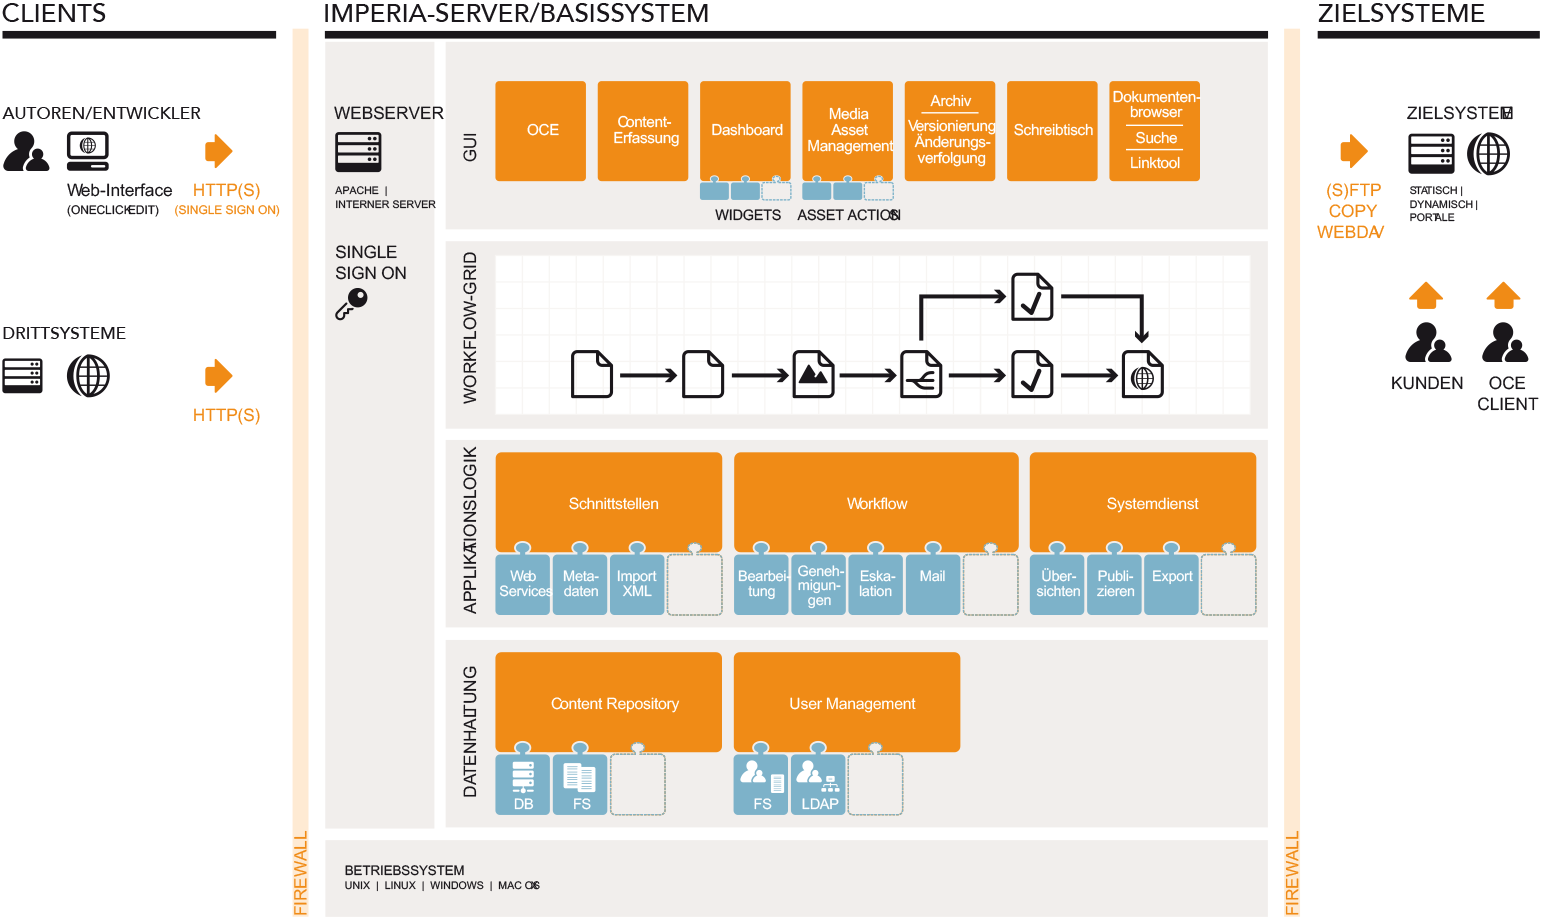
\includegraphics[width=\textwidth]{../resources/imperia/architektur.png}
            \caption{Architkektur von {\imperia} \cite{imperia:ecmd}}
            \label{image:imperiaArchitektur}
        \end{figure}

        Die wichtigste Komponente in dieser Architektur ist der imperia Server,
        der die zentralen Funktionen des Systems bereitstellt.
        Dazu gehören das Anlegen und Strukturieren von Projekten
        und Dokumenten sowie die Ausführung von Workflows.
        Außerdem verwaltet er die Datenhaltung.

        Die verschiedenen Nutzer des Systems
        verwenden für ihre Arbeit eine Weboberfläche,
        die über HTTP(S) mit dem Server kommuniziert.
        Über das gleiche Protokoll können auch Drittsysteme den Server
        ansprechen und verschiedene Aktionen durchführen oder Daten abfragen.

        Sobald ein Dokument alle Workflow-Schritte durchlaufen hat,
        wird es durch eine automatische oder manuelle Publizierung
        in eine Datei generiert, die dann auf ein Zielsystem übertragen wird.
        Dieses System ist eigenständig und gehört nicht zu {\imperia}.
        Allerdings bietet es die Möglichkeit über Dienste wie (S)FTP
        die generierten Dateien zu empfangen.
        Ein Beispiel sind Webserver, auf die Webseiten publiziert werden,
        die sie dann Besuchern bereitstellen.
    \section{\wordpress}
    % TODO:
    % - Sites!!!
    \label{section:WordPress}
    Das Open-Source-Projekt {\wordpress} startete 2003
    mit dem Ziel eine Anwendung zur einfachen Pflege eines Weblogs
    (kurz Blog) zu schaffen \cite{wordpress:About}.
    Das Ergebnis ist die gleichnamige Software,
    die noch immer von der Community weiterentwickelt
    und von der Fakultät \gls{ksw} der {\fernUni} für ihren
    Internetauftritt genutzt wird.
    In diesem Kapitel werden grundlegende Konzepte dieses Systems vorgestellt.

    \subsection{Weblog-Software}
        \label{section:weblogSoftware}
        {\wordpress} ist im Kern eine Software zur Pflege eines Blogs,
        wobei es sich um eine spezielle Form einer Webseite handelt
        \cite[Kapitel "`Introduction to Blogging"']{wordpress:codex}:

        \begin{quote}
            "`Blog"' is an abbreviated version of "`weblog"',
            which is a term used to describe websites that maintain
            an ongoing chronicle of information.
            A blog features diary-type commentary and links to articles
            on other websites, usually presented as a list of entries in
            reverse chronological order.
            Blogs range from the personal to the political,
            and can focus on one narrow subject or a whole range of subjects.
        \end{quote}

        Da Blogs eine spezielle Form von Webseiten sind,
        kann man auch eine Anwendung zu ihrer Pflege als
        spezielle Form eines \glspl{cms} betrachten.
        Diese Aussage trifft {\wordpress} auch über sich selbst
        und vergleichbare Software \cite[Kapitel "`Introduction to Blogging"']{wordpress:codex}:

        \begin{quote}
            Many blogging software programs are considered a specific type of CMS.
            They provide the features required to create and maintain a blog,
            and can make publishing on the internet as simple as writing an article,
            giving it a title, and organizing it under (one or more) categories.
        \end{quote}

        Nicht zuletzt, weil auch Privatpersonen eine Zielgruppe
        solcher Anwendungen sind, vereinfachen sie Blogeinträge
        auf die zwei elementaren Elemente Titel und Inhalt.
        Mit dieser schwachen Strukturierung der Inhalte
        unterscheidet sich {\wordpress} deutlich von {\imperia}
        und seinen Dokumenten, die beliebig stark strukturiert
        werden können.
        Aufgrund der Anpassbarkeit durch Themes
        und Plugins sieht sich
        {\wordpress} trotzdem als vollwertiges \gls{cms}
        \cite{wordpress:About}.

    \subsection{Dynamische Generierung}
        \label{section:problemAnalysisWordPressDynamicGeneration}
        Anders als {\imperia} ist {\wordpress} nicht nur das Redaktionssystem,
        sondern gleichzeitig auch das ausliefernde Zielsystem.
        Inhalte generiert {\wordpress} deshalb nicht in statische Dateien,
        sondern erzeugt eine Webseite auf Anfrage dynamisch.

    \subsection{Posts und Pages}
        \label{section:wordpressPostsPages}
        {\wordpress} unterscheidet zwei Arten von Beiträgen \cite[Kapitel "`Pages"']{wordpress:codex},
        auf denen eine Webseite basieren kann: Posts
        und Pages.

        \paragraph*{Posts}
        Klassische Blogeinträge werden in {\wordpress} "`Posts"' genannt.
        Neben der Pflege des Titels und des Inhaltes eines Posts stehen dem
        Anwender noch weitere Optionen zur Verfügung.
        Ein Post kann in Kategorien einsortiert oder mit Schlagwörtern versehen werden.
        Dadurch kann {\wordpress} Übersichtsseiten generieren,
        die z. B. alle Posts einer Kategorie enthalten.
        Über den eigentlichen Inhalt hinausgehende Informationen können
        in sogenannten "`Custom Fields"' gespeichert werden.
        Davon machen z. B. Plugins Gebrauch
        und speichern Metadaten des Posts in ihnen.
        Jeder Post besitzt einen Post Type,
        der eine Aussage über die Art des Beitrages macht.
        {\wordpress} definiert einige Standardtypen \cite[Kapitel "`Post Types"']{wordpress:codex},
        lässt aber auch die Angabe eigener Typen zu.
        Die Standardtypen sind:

        \begin{itemize}
            \item Post,
            \item Page,
            \item Attachment,
            \item Revision,
            \item Navigation Menu,
            \item Custom CSS und
            \item Changesets.
        \end{itemize}

        Der Typ eines Posts ändert nichts an seinen redaktionellen Feldern.
        Das heißt, unabhängig vom Post Type besitzt ein Beitrag nur
        einen Titel und Inhalt
        \cite[Kapitel "`Posts"' \& "`Post Types"']{wordpress:codex}.
        Stattdessen machen Typen wie Revision und Custom CSS deutlich,
        dass {\wordpress} Posts auch zur Realisierung technischer Anforderung verwendet.

        \paragraph*{Pages}
        Neben Posts kennt {\wordpress} auch das Konzept einer Page \cite[Kapitel "`Pages"']{wordpress:codex},
        die sich in ihrem Zweck klar von einem Post unterscheidet:

        \begin{quote}
            In contrast, pages are generally for non-chronological,
            hierarchical content: pages like "`About"' or "`Contact"'
            would be common examples.
            [...]
            Pages live outside of the normal blog chronology,
            and are often used to present timeless information about
            yourself or your site -- information that is always relevant.
            You can use Pages to organize and manage the structure of your website content.
        \end{quote}

        Aus diesem Grund besitzen Pages zwar ebenfalls einen Titel und Inhalt,
        können aber lediglich mit Schlagwörtern versehen werden.
        Die Einordnung in eine Kategorie ist nicht möglich
        \cite[Kapitel "`Pages"']{wordpress:codex}.
        Wie aus der oben erfolgten Auflistung der Post Types hervorgeht,
        sind Pages technisch gesehen lediglich Posts mit dem Post Type "`Page"'.

        {\wordpress} speichert alle Inhalte in einer relationalen Datenbank \cite[Kapitel "`Database Description"']{wordpress:codex}.
        Posts und Pages teilen sich in dieser Datenbank eine Tabelle,
        was ebenfalls verdeutlicht, dass Pages lediglich Posts eines speziellen Typs sind.
        Der Inhalt eines Beitrages wird in der Datenbank als \gls{html}-Fragment abgelegt,
        welches während der dynamischen Generierung in die Webseite übernommen wird.
        Zusätzlich enthält ein Beitrag aber auch spezielles Anweisungen\footnote{vgl. Kapitel \ref{section:wordpressPlugins}},
        welches von {\wordpress} während der Generierung interpretiert wird.

    \subsection{Vorlagen und Themes}
        \label{section:wordpressTemplatesThemes}
        Wie {\imperia} strebt auch {\wordpress} eine Trennung von
        Inhalt und Layout an.
        Inhalte werden dazu in
        Posts und Pages
        unabhängig vom Layout der Webseite gespeichert.
        Das Layout bestimmen Vorlagen und Themes.

        \paragraph*{Vorlagen}
        {\wordpress} nutzt Vorlagen \cite[Kapitel "`Templates"']{wordpress:codex}, um Inhalte in eine Seite einzubinden
        und ihr Aussehen festzulegen.
        Dazu definieren sie das Gerüst der Webseite und enthalten Kommandos,
        um Inhalte aus der Datenbank auszulesen.
        Eine Webseite wird auf Basis einer Vorlage dynamisch von {\wordpress} generiert.
        Vorlagen sind bei genauerem Hinsehen nichts anderes als PHP-Dateien,
        die \gls{html}, allgemeinen PHP-Code und sogenannte
        "`Template-Tags"' enthalten.
        Dabei handelt es sich um Aufrufe von
        {\wordpress}-eigenen PHP-Funktionen,
        um Inhalte aus der Datenbank abzufragen.
        Während der Generierung -- technisch lediglich die Ausführung
        des PHP-Codes -- können Vorlagen andere Vorlagen inkludieren,
        wodurch wiederkehrende Elemente in eigene Vorlagen ausgelagert
        werden können \cite[Kapitel "`Template Files"']{wordpress:codex}.
        Anhand der \gls{url} der Anfrage und der darin enthaltenen
        Kennung eines Posts oder einer Page,
        entscheidet {\wordpress}, welche Vorlage es zur Generierung der Seite nutzt
        \cite[Kapitel "`Template Hierarchy"']{wordpress:codex}.

        \paragraph*{Themes}
        Eine Sammlung aller {\resources}, die notwendig sind, um
        eine Webseite und ihr Layout umzusetzen,
        wird im Kontext von {\wordpress} als "`Theme"' bezeichnet.
        Ein Theme enthält demnach Vorlagen, Bilder sowie
        JavaScript-, \gls{css}-, und PHP-Dateien.
        Themes können {\resources} anderer Themes wiederverwenden oder überschreiben,
        wodurch Anpassungen an einem vorhandenen Theme einfach umzusetzen sind
        \cite[Kapitel "`Using Themes"']{wordpress:codex}.

    \subsection{Plugins}
        \label{section:wordpressPlugins}
        {\wordpress} besitzt ein Plugin-System \cite[Kapitel "`Plugins"']{wordpress:codex},
        über das es beliebig funktional erweitert werden kann,
        ohne an {\wordpress}' eigenen Quellen Änderungen vorzunehmen.
        Es existiert eine große Anzahl an freien Plugins,
        die oft benötigte Funktionen implementieren.
        Meist sind dies Funktionen, die über eine reine Weblog-Software hinausgehen.
        Ein Beispiel ist das Plugin
        "`Form Maker"'\footnote{vgl. \url{https://wordpress.org/plugins/form-maker/}},
        welches die Definition von Webformularen erlaubt,
        die dann in beliebigen Beiträgen eingebettet werden können.
        Zur Nutzung eines Plugins wird meist eine spezielle Anweisung -- ein Shortcode \cite[Kapitel "`Shortcode API"']{wordpress:codex} --
        in den Inhalt eines Posts oder einer Page geschrieben,
        die zum Zeitpunkt der Generierung ausgewertet wird.
        Beim Form Maker Plugin wäre dies zum Beispiel \texttt{[Form id="1"]},
        wodurch das Formular mit der Kennung "`1"' in die Webseite integriert wird.

    \section{Eine Migration von {\wordpress} zu {\imperia}}
    An einem Beispiel soll erklärt werden,
    wie eine manuelle Migration der Inhalte einer Webseite von {\wordpress} zu {\imperia}
    vonstatten gehen könnte und wo die größte Herausforderung dabei liegt.
    Darauf basierend erklärt das nächste Kapitel,
    welchem Aspekte dieses Prozesses sich diese Arbeit widmet.

    Als Beispiel dient die Seite eines Mitarbeiters,
    die schon aus Kapitel \ref{section:fernUniChallenges} bekannt ist.
    Die Schritte, die ein {\editor} zur Migration dieser Seite durchführen muss,
    sind schnell beschrieben:

    \begin{enumerate}
        \item   Der {\editor} öffnet die Seite des Mitarbeiters in {\wordpress}.
        \item   Der {\editor} legt in {\imperia} ein neues Dokument an.
                Die Wahl einer Vorlage trifft er autonom oder nach festgelegten Kriterien.
        \item   \label{item:problemAnalysisManualMigrationSlectInfoStep}Der {\editor} kopiert den Namen, die Telefonnummer und die E-Mail-Adresse
                des Mitarbeiters einzeln aus dem gemeinsamen Formularfeld in {\wordpress}
                und fügt sie in die vorgesehenen Felder in {\imperia} ein.
                Welche dies sind entscheidet er wiedrum autonom oder aufgrund einer Regel.
        \item   Der {\editor} lädt das Bild des Mitarbeiters von {\wordpress} herunter
                und fügt es in {\imperia} ein.
        \item   Der {\editor} füllt bei Bedarf sonstige Felder in {\imperia},
                für die es in {\wordpress} keine Entsprechung gab.
        \item   Der {\editor} speichert das Dokument und gibt es frei.
    \end{enumerate}

    Prinzipiell kann jeder dieser Schritte über die Schnittstellen von {\wordpress}
    und {\imperia} durch passende Migrationsskripte automatisiert werden.
    Lediglich der \ref{item:problemAnalysisManualMigrationSlectInfoStep}. Schritt
    birgt eine konzeptionelle Herausforderung für eine Automatisierung.
    Nämlich, wie ein Migrationsskript entscheiden soll, was im Formularfeld in {\wordpress}
    der Name, was die Telefonnummer und was die E-Mail-Adresse des Mitarbeiters ist.
    Alles steht in einem gemeinsamen Formularfeld, weshalb die Informationen nicht
    einzeln angesprochen werden können.
    Vor allem unter dem Gesichtspunkt, dass das Feld ein Freitextfeld ist und prinzipiell beliebig gefüllt sein kann.
    Ein Mensch kann diese Zuordnung leicht treffen,
    eine Maschine muss hingegen instrumentiert werden.

    \section{Klassifizierung der Inhalte einer Webseite}
    \label{section:WebpageClassification}
    Kapitel \ref{section:fernUniChallenges}
    ist bereits auf das Vorhaben der {\fernUni}
    eingegangen, die {\wordpress}-basierten Seiten der Fakultät
    \gls{ksw} zu {\imperia} zu migrieren.
    Ein Vergleich der in den Kapiteln
    \ref{section:Imperia} und \ref{section:WordPress} vorgestellten
    Datenstrukturen dieser Systeme verdeutlicht die Herausforderung bei diesem
    Vorhaben.
    {\wordpress} speichert die Inhalte einer Seite unstrukturiert in einem einzigen Feld,
    wohingegen {\imperia} eine höhere Strukturierung der Inhalte vorsieht.
    Eine Überführung der Inhalte in die feineren Strukturen von
    {\imperia}, wie es die Universität beabsichtigt
    \footnote{vgl. Kapitel \ref{section:fernUniChallenges}},
    ist also nicht ohne Weiteres möglich.

    Aus diesem Grund soll die Möglichkeit einer automatischen
    Klassifizierung der Inhalte untersucht werden,
    deren Ergebnis die beschriebene Migration vereinfachen würde.
    Dieses Kapitel verfeinert diese Aufgabenstellung und klärt folgende Fragen:

    \begin{enumerate}
        \item Welche Elemente einer Webseite sind für eine Klassifizierung interessant?
        \item Nach welchen Kriterien findet eine Klassifizierung statt?
        \item Welche allgemeinen Anforderungen ergeben sich daraus?
    \end{enumerate}

    Die in den vorangegangenen Kapiteln gewonnenen Erkenntnisse ermöglichen
    die Beantwortung dieser Fragen.
    Zur Veranschaulichung wird unter anderem eine Seite der Fakultät \gls{ksw}
    \footnote{\url{http://www.fernuni-hagen.de/KSW/portale/babw/service/}, Stand 01.02.2018}
    herangezogen.
    Abbildung \ref{image:BaBwFAQ} zeigt einen Ausschnitt dieser
    Seite, der den Inhalt des Beitrages in {\wordpress} widerspiegelt.

    \begin{figure}
        \centering
        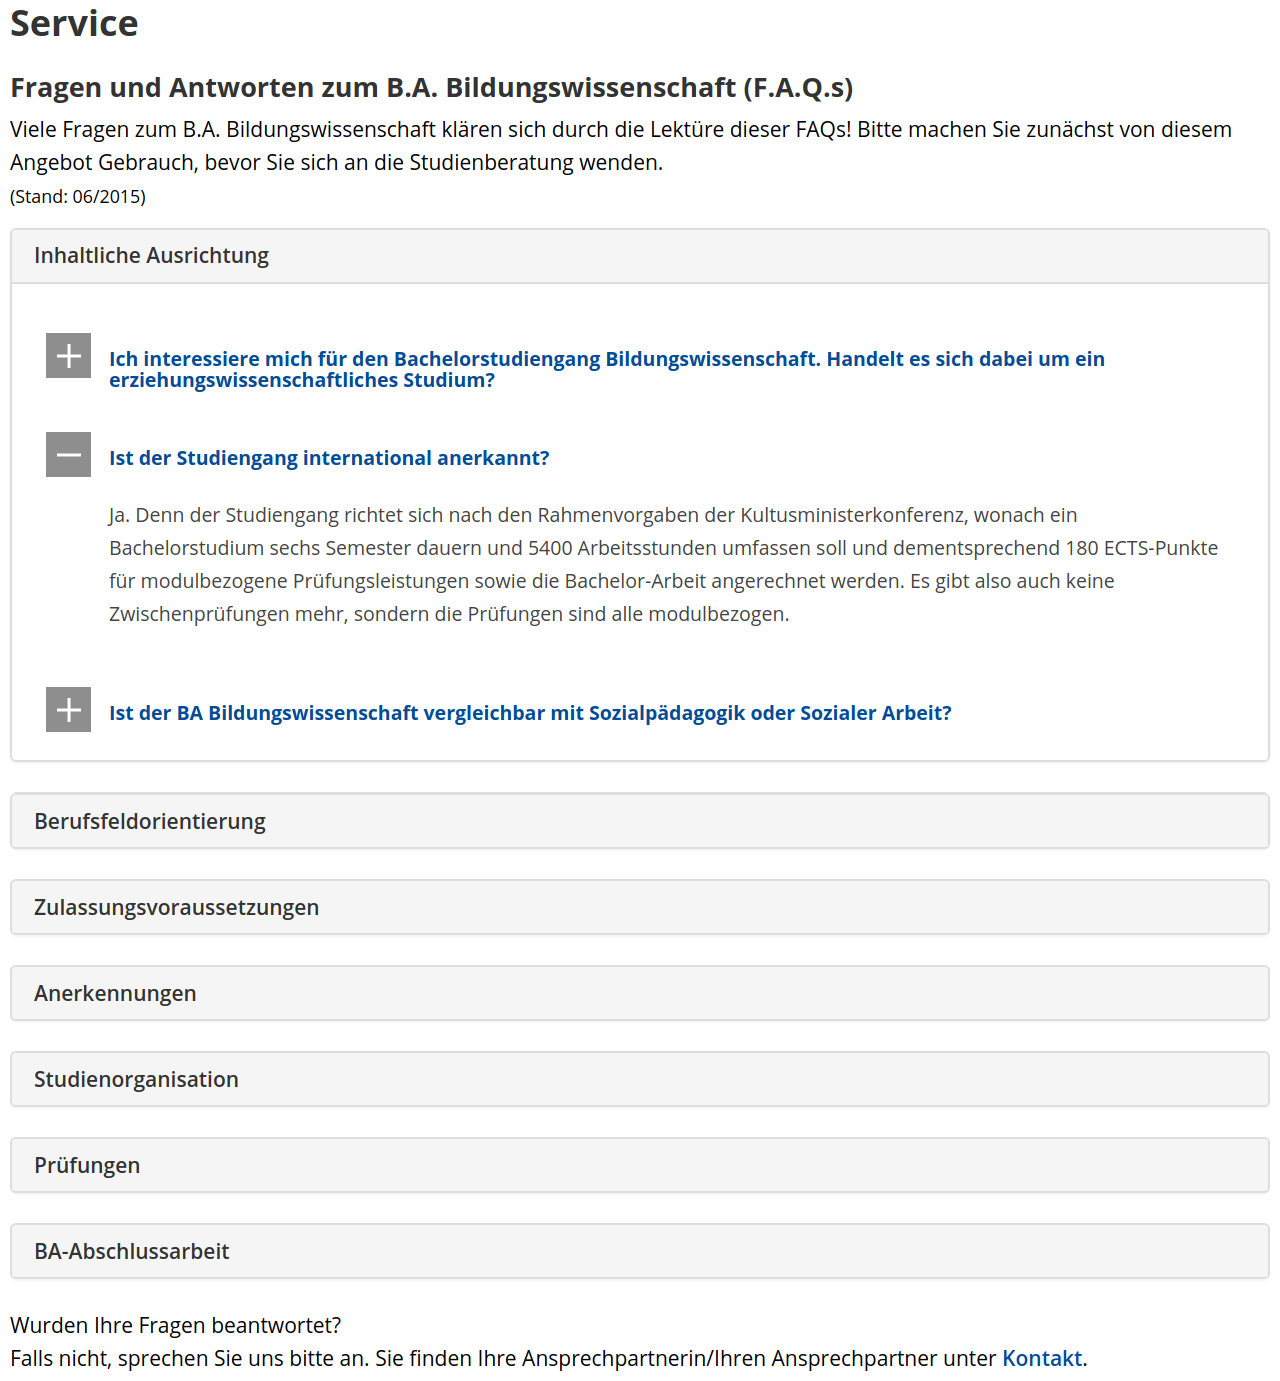
\includegraphics[width=\textwidth]{../resources/babw_service_faq.png}
        \caption{F.A.Q. Seite des Studienportals "`B.A. Bildungswissenschaft"'}
        \label{image:BaBwFAQ}
    \end{figure}

    Diese Seite beinhaltet Anworten zu häufig gestellten Fragen
    zum \gls{babw}.

    \subsection{Relevante Entitäten}
        \label{section:classificationEntities}
        Die Anforderung die Inhalte einer Seite zu klassifizieren
        ist allgemein und lässt die Frage offen,
        welche Bestandteile einer Seite hierfür von Bedeutung sind.
        Dieser Frage soll sich über die konkrete Anforderung
        der {\fernUni} genähert werden.

        Würde man manuell eine aus {\wordpress} stammende Seite zu
        {\imperia} migrieren, stellten sich mindestens drei Fragen:

        \begin{enumerate}
            \item   Auf welcher Vorlage soll die Seite basieren?
                    Das heißt zu welcher Kategorie gehört sie?
            \item   Mit welchen Inhalten sind die unterschiedlichen Felder
                    des Formulares zu füllen?
            \item   Welcher Bilder, Videos und Links auf andere Seiten existieren,
                    und wie müssen sie in die neue Seite übernommen werden?
        \end{enumerate}

        Am leichtesten ist die zweite Frage zu beantworten.
        Die Felder werden selbstverständlich mit dem Inhalt des Beitrages
        aus {\wordpress} gefüllt.
        Diese textuellen Inhalte müssen folglich einer Klassifizierung unterzogen werden.
        
        Im einfachen Fall basiert jede migrierte Seite in {\imperia} auf derselbe Vorlage.
        Es ist allerdings nicht unwahrscheinlich,
        dass verschiedene Layouts und damit verschiedene Vorlagen
        notwendig werden.
        Die Wahl der Vorlage wird dann auf der originalen Seite basieren,
        weshalb auch die Klassifizierung einer Seite als Ganzes notwendig ist.
        Jeder Klasse wird anschließend eine Kategorie in {\imperia}
        zugewiesen, die wiederum die zu nutzende Vorlage bestimmt.
        Eine Klassifizierung der gesamten Seite kann außerdem die
        Klassifikation der Inhalte in einen Kontext setzen.
        Die Klasse "`Frage"' auf der F.A.Q-Seite des \gls{babw}
        ist zum Beispiel aussagekräftiger, wenn bekannt ist,
        dass die Seite zur Klasse "`F.A.Q."' gehört.

        Die dritte Frage besteht aus zwei Teilen.
        Der erste Teil fragt allgemein gesprochen nach einer Auflistung referenzierter {\resources},
        deren Bereitstellung keine Herausforderung darstellt,
        da sie direkt aus dem \gls{html}-Dokument hervorgeht.
        Der zweite Teil zielt hingegen darauf ab,
        wie sich die jeweilige {\resource} und die Referenz selbst einordnen lassen.
        Bilder, Videos und Links werden in der neuen Seite selbstverständlich
        unterschiedlich eingebunden.
        Das Banner einer Seite -- technisch ebenfalls nur ein Bild --
        besitzt womöglich ein dediziertes Eingabefeld,
        weshalb auch innerhalb der Gruppe "`Bilder"' weiter unterteilt werden muss.
        Das gilt zum Beispiel auch für Links.
        Referenzen auf externe Seiten erhalten häufig ein anderes Layout als Links
        auf Seiten innerhalb der eigenen Site.
        Referenzen müssen demnach ebenfalls klassifiziert werden.

        Zusammengefasst lassen sich also drei Entitäten ermitteln,
        die für eine Klassifizierung relevant sind:
        Die Seite als Ganzes, textueller Inhalt und Referenzen.

    \subsection{Kriterium der Klassifizierung}
        \label{section:ClassificationCriteria}
        Nachdem nun geklärt ist, welche Entitäten einer Webseite für
        eine Klassifizierung relevant sind\footnote{vgl. Kapitel \ref{section:classificationEntities}},
        widmet sich dieses Kapitel der Frage, nach welchen
        Kriterien diese Einordnung erfolgen muss
        und welche Bedeutung die resultierenden Klassen besitzen.

        Die Klassifikation der Seite hat direkten Einfluss auf die Wahl der Vorlage im neuen \gls{cms}.
        Die Klasse der Seite könnte auf dem Typ des Beitrages basieren,
        also ob er ein Post oder eine Page ist.
        In der Praxis wird diese Unterteilung aber nicht ausreichen,
        da verschiedene Pages im Zielsystem verschiedene Layouts erhalten werden.
        Eine fachliche Unterteilung der Seiten anstatt einer technischen ist deshalb sinnvoller.
        Für die F.A.Q.-Seite des \gls{babw} hieße das zum Beispiel,
        dass sie als "`FAQ-Seite"' klassifiziert wird und nicht als "`Page"'.
        Eine fachliche Unterscheidung nach inhaltlicher Bedeutung macht die
        gewonnene Klassifikation außerdem unabhängiger vom konkreten
        Migrationsvorhaben und somit für andere Anwendungsfälle nutzbar.

        Die Einteilung von Referenzen und textueller Inhalte kann ebenfalls
        mit einer technischen oder fachlichen Ausrichtung erfolgen.
        Technisch ließen sich Inhalte zum Beispiel anhand ihres \gls{html}-Elementes einteilen.
        Es entstünden also Klassen wie "`p"', "`h1"' usw.
        Auf der F.A.Q.-Seite des \gls{babw} fände sich der einleitende Text vor dem
        ersten Themenbereich in der Klasse "`p"' wieder.
        Das gleiche gilt für den abschließenden Textabsatz nach dem letzten Themenbereich.
        Falls in {\imperia} zu diesen Absätzen
        korrespondierende Felder existieren, kann ein Automatismus basierend auf dieser
        Klassifikation nicht entscheiden, welches Feld mit welchem Inhalt zu füllen ist.
        
        Eine Einteilung nach Layoutelementen ist ebenso wenig hilfreich.
        Im beschriebenen Fall hieße die Klasse dann nämlich nicht "`p"',
        sondern "`Text"', was die Füllung der Felder nicht vereinfacht.
        Ein weiteres Beispiel sind die aufklappbaren Elemente auf der Seite,
        die sich nach diesem Konzept
        der Klasse "`Accordion"'\footnote{vgl. \url{https://getbootstrap.com/docs/3.3/javascript/\#collapse-example-accordion}}
        zuweisen ließen.
        Die Information, dass Inhalte ein gewisses Layout verwenden,
        ist unbrauchbar, wenn nicht gewährleistet ist,
        dass alle diese Inhalte wieder dieses Layout verwenden werden.

        Abhilfe bringt wiederum nur eine fachliche Klassifizierung,
        bei der die inhaltliche Bedeutung im Vordergrund steht.
        Das heißt anstelle von allgemeinen Klassen wie "`p"', "`Text"'
        oder "`Accordion"', sind spezifischere fachliche Klassen wie
        "`Einleitung"', "`Schluss"', "`FAQ-Themenbereich"', "`Frage"' und "`Antwort"'
        notwendig.
        Nur so lässt sich entscheiden, wie die Inhalte in das neue \gls{cms}
        zu überführen sind.

        Diese Schlussfolgerung gilt auch für Referenzen.
        Das Banner einer Seite kann nicht als "`img"'
        oder als "`Carousel"'\footnote{vgl. \url{https://getbootstrap.com/docs/3.3/javascript/\#carousel}}
        klassifiziert werden, weil immer die Möglichkeit besteht,
        dass aufgrund dieser technischen Einteilung nicht klar wird,
        wie die Inhalte der Seite zu übertragen sind.
        Benötigt wird stattdessen die fachliche Information,
        dass die referenzierte {\resource} das Banner der Seite darstellt,
        weshalb die Referenz auch als "`Banner"' klassifiziert werden muss.

    \subsection{Anforderungen}
        \label{section:requirements}
        Die vorliegenden Informationen erlauben
        die Ableitung ausreichend konkreter Anforderungen,
        um die Problemstellung zu formulieren, der sich diese Arbeit widmet.

        \paragraph*{Automatisierte fachliche Klassifizierung von Seiten, Inhalten und Referenzen}
        Es ist ein System zu entwickeln, welches automatisiert Webseiten,
        deren Inhalte und Referenzen auf andere {\resources} im \gls{www}
        nach fachlichen und inhaltlichen Kriterien klassifiziert.
        Eine Klassifikation ermöglicht im vorliegenden konkreten Fall
        der {\fernUni} eine \gls{cms}-Migration von {\wordpress} zu {\imperia}.
        Allgemein erlaubt sie die Verarbeitung und Analyse der Webseiten.

        \paragraph*{Abbildung inhaltlicher Strukturen}
        Eine fachliche Klassifizierung bedeutet nicht,
        dass das Ergebnis aus einelementigen Klassen besteht.
        Die F.A.Q.-Seite des \gls{babw} enthält mehrere aufklappbare
        Themenbereiche (Inhaltliche Ausrichtung, Berufsfeldorientierung, etc.),
        die jeweils als "`FAQ-Themenbereich"' klassifiziert werden können.
        Des Weiteren enthält jeder Themenbereich mehrere Paare aus Frage und Antwort.
        Aus der Klassifikation muss entsprechend hervorgehen,
        welche Frage-Antwort-Paare zu welchem Themenbereich gehören,
        da diese Zuordnung Nutzer der Klassifikation nicht sicher vornehmen können.
        Daraus ergibt sich folgende allgemeine Anforderung:

        Eine Klassifikation muss die fachliche Struktur
        und Hierarchie der Inhalte widerspiegeln,
        um diese Zuordnung vor allem bei sich wiederholenden Strukturen
        nicht zu verlieren.
        Das heißt, besteht ein Inhalt $I$ fachlich aus den Inhalten $I_1 \ldots I_n$
        und den Referenzen $R_1 \ldots R_m$,
        muss die Klassifikation $I'$ von $I$ auch aus den Klassifikationen
        $I'_1 \ldots I'_n$ und $R'_1 \ldots R'_m$ bestehen.

        \paragraph*{Allgemeine Klassendefinition}
        Es muss möglich sein die fachlichen Klassen allgemein zu
        spezifizieren, sodass eine beliebige Anzahl an gegebenen
        Webseiten auf Basis dieser Spezifikation klassifiziert wird.
        Die Syntax einer solchen Spezifikation soll auch von Nutzern ohne
        Programmierkenntnisse verstanden werden können.

        \paragraph*{Schnittstelle zum Starten einer Klassifizierung}      
        Das System muss programmatisch angewiesen werden können,
        eine oder mehrere gegebene Webseiten zu klassifizieren,
        sodass ein Drittsystem die relevanten Webseiten auffinden
        und weitergeben kann.
        Der Aufwand einer manuellen Instrumentierung des Systems ist
        vor allem bei vielen Webseiten nicht zu rechtfertigen.

        \paragraph*{Schnitstelle zur Abfrage der Klassifikation}
        Die Klassifikation muss über eine definierte allgemeine
        Schnittstelle abrufbar sein, sodass Drittsysteme die Ergebnisse
        nutzen können.
        Im Fall der {\fernUni} könnte dies ein Werkzeug sein,
        welches die Migration von {\wordpress} zu {\imperia}
        durchführt und dafür auf die Klassifikation zurückgreift.

        \paragraph*{Möglichkeit der Nachbesserung}
        % TODO: Was ist die allgemeine Anforderung für:
        % Seiten sollen als "veraltet" markiert werden können, um sie von der Migration auszuschließen.
        Das System muss die Prüfung sowie die manuelle Nachbesserung
        des Klassifizierungsergebnisses erlauben,
        um Fehler zu erkennen und zu beheben.
        Das entsprechende Werkzeug soll eine graphische Benutzeroberfläche
        besitzen, um seine Nutzung möglichst einfach zu gestalten.

        \paragraph*{Allgemeingültigkeit}
        Trotz dem konkreten Anwendungsfall an der {\fernUni}
        soll ein allgemein nutzbares System entstehen,
        welches nicht auf die speziellen Anforderungen dieser Universität
        zugeschnitten ist.
        Das bedeutet, dass eine Klassifizierung von Webseiten außerhalb
        der {\fernUni} möglich sein muss.
        Außerdem, dass das System nicht annehmen darf,
        dass eine zu klassifizierende Webseite auf {\wordpress} basiert.

